\documentclass{ximera}

% \input{../../xmpreamble.tex}

\title{Activity: Introduction to Multivariable Functions}
\author{Zack Reed}

\begin{document}
\begin{abstract}
In this activity we explore functions with multiple variable inputs and single-variable outputs.
\end{abstract}
\maketitle

\section*{Introduction: From Vector Functions to Multivariable Functions}

After analyzing vector functions (where we input one variable and output a vector), we now examine scalar functions that have multiple input variables. These \emph{multivariable} functions are fundamental to conceptualizing the complexities of the world around us.

\subsection*{Review: What is a Function?}

Let's review some terminology from single-variable functions.

\begin{definition}
For a single-variable function $y = f(x)$, at each $x$-value we have a \textbf{single} assigned $y$-value. We say:
\begin{itemize}
    \item $x$ is the \textbf{input} (independent variable)
    \item $y = f(x)$ is the \textbf{output} (dependent variable)
    \item The graph is all of the pairs $(x, y) = (x, f(x))$ that link the input to the output
\end{itemize}

The variable $y$ \emph{depends on} $x$ because you can alter the $y$-value by altering the $x$-value.
\end{definition}

\begin{problem}
For a function $y = f(x)$, which statements are true? (Select all that apply.)

\begin{selectAll}
    \choice[correct]{Each $x$-value produces exactly one $y$-value}
    \choice{Each $y$-value comes from exactly one $x$-value}
    \choice[correct]{Multiple $x$-values can produce the same $y$-value}
    \choice[correct]{$y$ depends on $x$}
    \choice[correct]{Changing $x$ changes $y$}
\end{selectAll}

\begin{feedback}
The key property of a function is that each input produces exactly one output. However, multiple inputs can produce the same output! For example, $f(x) = x^2$ gives $f(-2) = f(2) = 4$.
\end{feedback}
\end{problem}

The following video reviews these ideas.

\begin{center}
\youtube{GU5ZZwQqrQQ}
\end{center}

\begin{problem}
Now visualize this concept with an interactive example.

\begin{expandable}{stuff}{GeoGebra Instructions}
    Alter the ``x='' slider to view different points on the graph of $f(x) = \sin(x) + \frac{x}{5}$. Notice how the input $x$ gives the horizontal component and the output $f(x)$ gives the vertical component of each point $(x,y)$.
\end{expandable}

\begin{center}
\geogebra{mvpqg764}{739}{456}
\end{center}

After exploring the applet, answer: As you move the slider, what primarily controls the change in $y$?

\begin{multipleChoice}
    \choice{The $y$-value changes randomly}
    \choice[correct]{The $y$-value changes because we slide the $x$-value}
    \choice{The $y$-value stays constant}
    \choice{Both $x$ and $y$ are independent}
\end{multipleChoice}

Complete the following expressions detailing the relationship between $x$ and $y$ and the graph of $f$:

\begin{enumerate}
    \item $f(3)$ is the \wordChoice{\choice{input}\choice[correct]{output}} when $x = 3$. $f(3)$ has a value of approximately $\answer[tolerance=.05]{.74}$. Its value is represented by the length of the \wordChoice{\choice{horizontal green}\choice[correct]{vertical blue}}.
    \item The graph has a height of approximately $1.18$ at \wordChoice{\choice{zero}\choice{one}\choice{two}\choice[correct]{three}} input values because for each of these \wordChoice{\choice[correct]{$x$}\choice{$y$}}-values, $f(\answer{x}) \approx 1.18$. These input values are represented by the \wordChoice{\choice[correct]{horizontal green}\choice{vertical blue}} lines in the applet.
    \item The point $(9,2.22)$ is a(n) \wordChoice{\choice{input}\choice{output}\choice[correct]{neither an input nor an output}} value of the function. The point expresses the relationship that when $x = \answer{9}$, then $f(9) \approx \answer{2.22}$.
\end{enumerate}

\begin{feedback}
This is the essence of a function: we change $y$ by first changing $x$. The output depends on the input!
\end{feedback}
\end{problem}

\subsection*{Extending to Multiple Inputs}

Now we create relationships between three or more variables and require that one variable \emph{depends on} the other variables, making a function in the same way we defined single-variable functions.

\begin{problem}
Before seeing the definition, predict: If we have a function of two variables $x$ and $y$, how should we think about the output?

\begin{multipleChoice}
    \choice{The output is a pair of numbers}
    \choice[correct]{The output is a single number that depends on both $x$ and $y$}
    \choice{The output is a vector}
    \choice{The output is a curve}
\end{multipleChoice}

Also, thinking about the graph of such a function, what should it look like?

\begin{multipleChoice}
    \choice{A curve in 2D made of points $(x, y)$}
    \choice{A curve in 3D made of points $(x, y, z)$}
    \choice[correct]{A surface in 3D made of points $(x, y, z)$}
    \choice{A volume in 3D made of points $(x, y, z)$}
\end{multipleChoice}

\begin{feedback}
Just like single-variable functions produce a single output from one input, multivariable functions produce a single output from multiple inputs!
\end{feedback}
\end{problem}

\begin{definition}
For a function $z = f(x, y)$ of two variables:
\begin{itemize}
    \item We can freely change both $x$ and $y$ (independent variables)
    \item For each pair $(x, y)$ we get a \textbf{single} $z$-value: $z = f(x, y)$ (dependent variable)
    \item The graph comprises points $(x, y, z) = (x, y, f(x, y))$
    \item Any one $z$-value might be associated with multiple $(x, y)$ pairs
\end{itemize}

The values of $f$ can be visually interpreted as a height (hence $z$) defined at any point on the $xy$-plane.
\end{definition}

The following video will help unpack how we interpret surface visualizations of multivariable functions.

\begin{center}
\youtube{KGVmENvAoyU}
\end{center}

\begin{problem}
Now visualize a multivariable function with this interactive applet.

\begin{expandable}{stuff}{GeoGebra Instructions}
    The left screen shows the $xy$-plane, and the right screen shows the surface $z = f(x,y)$. Click and drag the point $(x,y)$ on either screen. You can also click and drag to rotate the 3D view and scroll to zoom. Use ``Reset 3D Zoom'' to return to the global view.
\end{expandable}

\begin{center}
\geogebra{krfy4jsw}{751}{652}
\end{center}

After exploring, identify what you observed (select all that apply):

\begin{selectAll}
    \choice[correct]{Both $x$ and $y$ can be changed independently}
    \choice[correct]{Changing either $x$ or $y$ changes the $z$-value}
    \choice{Only one variable can change at a time}
    \choice[correct]{The graph is a surface in 3D made of points $(x, y, z)$}
    \choice[correct]{Each $(x,y)$ pair produces exactly one $z$-value}
\end{selectAll}

The specific way that $z$ relates to $x$ and $y$ is given by the function equation $z = f(x,y)$. $f$ describes how to build $z$ from operations on $x$ and $y$.

\begin{feedback}
Just as in the single-variable case, we have a dependent-independent relationship. The primary difference is that we now have two separate variables, $x$ and $y$, that can both be altered to change the value of $z = f(x,y)$.

This forms the foundation of the rest of our study of multivariable calculus!
\end{feedback}
\end{problem}

\section*{Examples of Multivariable Functions}

Let's explore concrete examples of multivariable functions.

\subsection*{Example 1: Volume of a Cylinder}

\begin{problem}
The volume formula is $V = \pi r^2 h$, a function: $V(r, h) = \answer{\pi r^2 h}$ can describe the volume of a cylinder based on radius $r$ and height $h$ that defines the cylinder. Both $r$ and $h$ are independent variables that we can change freely, and the volume $V$ depends on both.

Use the following applet to explore the interactive visualization of the cylinder volume function. For the sake of visualization, the ``$x$-$y$ plane'' is shifted lower than in typical graphs.

\begin{expandable}{stuff}{GeoGebra Instructions}
    Use the sliders to adjust the radius and height. Watch how the cylinder's volume changes. Notice how the function depends on both variables simultaneously.
\end{expandable}

\begin{center}
\geogebra{vss2d9yc}{733}{520}
\end{center}

If a cylinder has radius $r = 3$ cm and height $h = 5$ cm:
$V(3, 5) = \pi \cdot (\answer{3})^2 \cdot \answer{5} = \answer{45}\pi$ cubic cm

If we double the radius: $V(6, 5) = \answer{180}\pi$ cubic cm

Doubling the radius \wordChoice{\choice{doubles the volume}\choice{triples the volume}\choice[correct]{quadruples the volume}} because radius is squared.



After exploring, answer: If you fix the height at $h=4$ and vary only the radius, the volume:
\begin{multipleChoice}
    \choice{Increases linearly with radius}
    \choice[correct]{Increases quadratically with radius}
    \choice{Increases cubically with radius}
    \choice{Remains constant}
\end{multipleChoice}

If you fix the radius at $r=2$ and vary only the height, the volume:
\begin{multipleChoice}
    \choice[correct]{Increases linearly with height}
    \choice{Increases quadratically with height}
    \choice{Increases cubically with height}
    \choice{Remains constant}
\end{multipleChoice}

\begin{feedback}
The volume is proportional to $r^2$ (quadratic in $r$) but proportional to $h$ (linear in $h$). This shows how the function responds differently to changes in different variables!

To evaluate $V(3,5)$, substitute $r=3$ and $h=5$. Both variables are needed to determine volume.
\end{feedback}
\end{problem}

\begin{remark}
    \textbf{Level Sets:} Often, because of software constraints or formatting issues, we cannot visualize full 3D surfaces. Instead, we can visualize \emph{level sets} (or \emph{contour plots}), which are curves in the $xy$-plane where the function takes on a constant value.

    That is, we find the 2D curves (or later 3D surfaces) where the function takes on a specific output value. This is akin to horizontally slicing 3D surfaces as we did in the last module. 

    As an example, the level sets of the cylinder volume function $V(r,h) = \pi r^2 h$ are given by fixing $V = k$ for some constant $k$:

    \begin{center}
    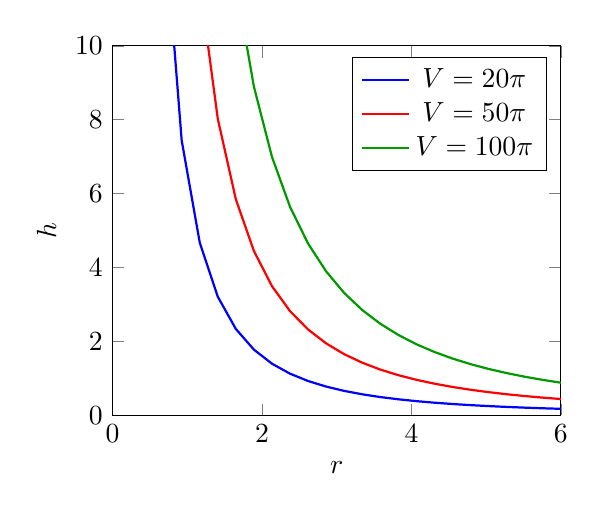
\begin{tikzpicture}
    \begin{axis}[xlabel=$r$, ylabel=$h$, xmin=0, xmax=6, ymin=0, ymax=10, width=0.6\textwidth, legend pos=north east]
    \addplot[blue, thick, domain=0.2:6] {20/(pi * x^2)}; \addlegendentry{$V=20\pi$}
    \addplot[red, thick, domain=0.2:6] {50/(pi * x^2)}; \addlegendentry{$V=50\pi$}
    \addplot[green!60!black, thick, domain=0.2:6] {100/(pi * x^2)}; \addlegendentry{$V=100\pi$}
    \end{axis}
    \end{tikzpicture}
    \end{center}

    Here, we're looking \textbf{at the domain} of the function. Remember, it's important to keep in mind where you're looking. This still gives us some information about the function's behavior and even what the surface might look like. We can see that the function takes on higher values as you move away from the origin, and there is an inverse square relationship between $r$ and $h$ for fixed volume.
\end{remark}

\subsection*{Example 2: Temperature on a Plate}

\begin{problem}
Consider a metal plate where the temperature (in degrees) at a point $(x,y)$ is given by
\[ T(x,y) = 100 - x^2 - y^2. \]

What this function means is that a $10\times 10$ square plate is in the first quadrant (where $0 \le x \le 10$ and $0 \le y \le 10$), and there is a heat source at the origin $(0,0)$ producing a maximum temperature of $100$ degrees. The temperature decreases as you move away from the origin, and the height of the surface represents the temperature at each point.

The surface of the function $z = T(x,y)$ over the box $0 \le x \le 10$, $0 \le y \le 10$ looks like the following:

\begin{center}
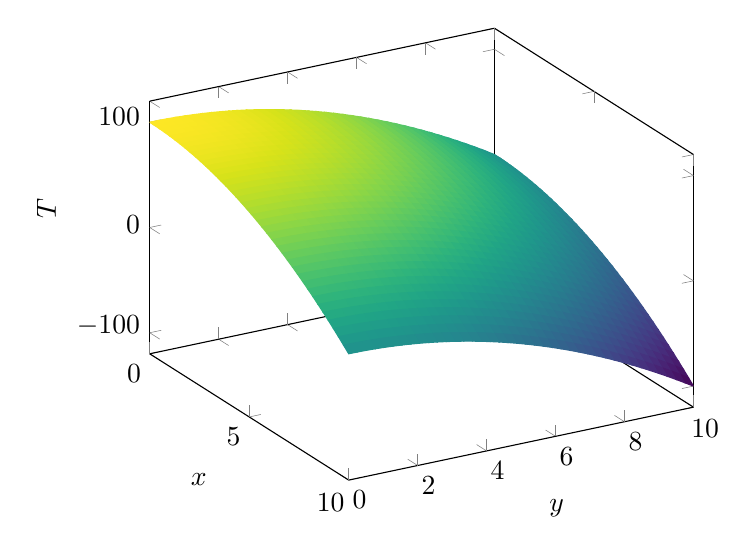
\begin{tikzpicture}
\begin{axis}[view={60}{30}, xlabel=$x$, ylabel=$y$, zlabel={$T$}, domain=0:10, y domain=0:10, colormap/viridis, samples=40, samples y=40, width=0.7\textwidth]
\addplot3[surf, shader=flat] {100 - x^2 - y^2};
\end{axis}
\end{tikzpicture}
\end{center}

The level curves of the temperature function $T(x,y)$ are given by fixing $T = k$ for some constant $k$:

\begin{center}
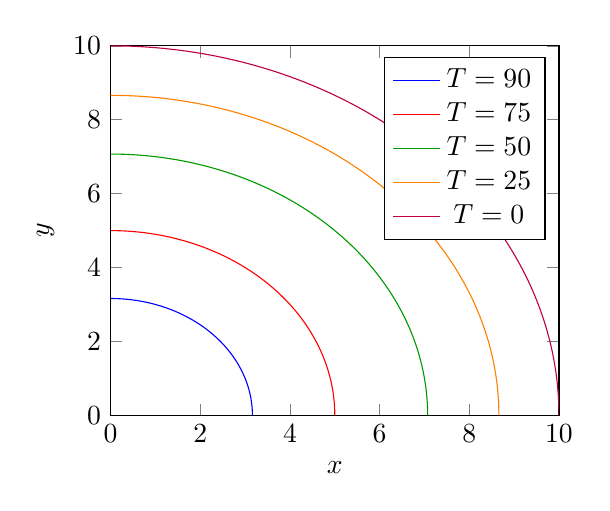
\begin{tikzpicture}
\begin{axis}[xlabel=$x$, ylabel=$y$, xmin=0, xmax=10, ymin=0, ymax=10, width=0.6\textwidth, legend pos=north east]
% Quarter-circles (contours) for T(x,y)=100-x^2-y^2
\addplot[blue, samples=200, domain=0:90] ({3.1623*cos(x)},{3.1623*sin(x)}); \addlegendentry{$T=90$}
\addplot[red, samples=200, domain=0:90] ({5*cos(x)},{5*sin(x)}); \addlegendentry{$T=75$}
\addplot[green!60!black, samples=200, domain=0:90] ({7.0711*cos(x)},{7.0711*sin(x)}); \addlegendentry{$T=50$}
\addplot[orange, samples=200, domain=0:90] ({8.6603*cos(x)},{8.6603*sin(x)}); \addlegendentry{$T=25$}
\addplot[purple, samples=200, domain=0:90] ({10*cos(x)},{10*sin(x)}); \addlegendentry{$T=0$}
\end{axis}
\end{tikzpicture}
\end{center}

Answer the following questions:

\begin{enumerate}
\item The maximum temperature in the domain $0\le x\le 10$ ,$0 \le y \le 10$ is $\answer{100}$ degrees at the point $(\answer{0},\answer{0})$.
\item $T(3,4)=\answer{75}$ degrees.
\item According to the level curves, the temperature at $(\frac{3\sqrt{2}}{2},\frac{3\sqrt{2}}{2})$ is $\answer{90}$ degrees. (Hint: Think about the level curves and the unit circle.)
\item The level curve $T=0$ is the \wordChoice{\choice{square}\choice{ellipsoid}\choice[correct]{circle}\choice{sphere}} defined by the equation $x^2 + y^2 = \answer{100}$ and is all points $(x,y)$ where the temperature is $\answer{0}$ degrees.
\end{enumerate}

\begin{feedback}
Remember that levels curves live in the domain, and are the sets of points $(x,y)$ where the function takes on a set, specific value. Here, the level curves are quarter-circles centered at the origin, showing how temperature decreases as you move away from the heat source.
\end{feedback}
\end{problem}

\subsection*{Example 3: Bacterial Growth (Nutrient × Time)}

\begin{problem}
A bacterial population is modeled by
\[ N(t,c) = c\,e^{0.5t}, \]
where $t$ is time (in hours) and $c$ is the initial nutrient level which scales the initial population.

Graph $N$ for small positive times (e.g., $0\le t\le 5$) and try several values of $c$ (for example $c=1,2,5$). Observe how changing $t$ and $c$ affects $N$.


\begin{center}
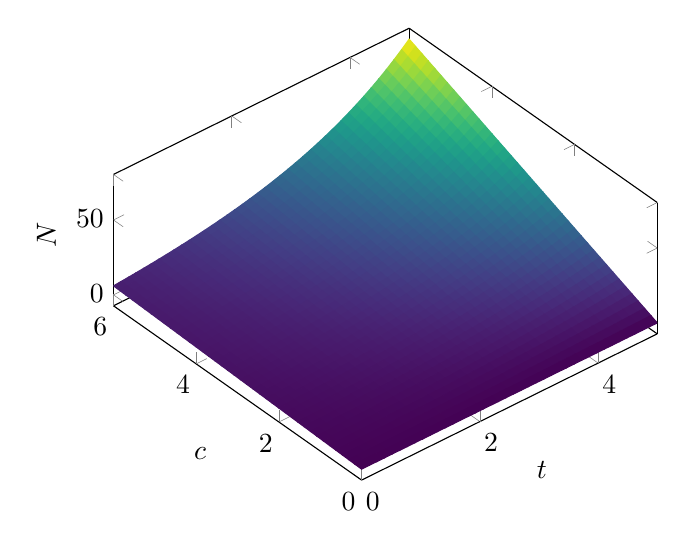
\begin{tikzpicture}
\begin{axis}[view={-40}{60}, xlabel=$t$, ylabel=$c$, zlabel={$N$}, domain=0:5, y domain=0:6, colormap/viridis, samples=40, samples y=40, width=0.7\textwidth]
\addplot3[surf, shader=flat] {y*exp(0.5*x)};
\end{axis}
\end{tikzpicture}
\end{center}

\begin{center}
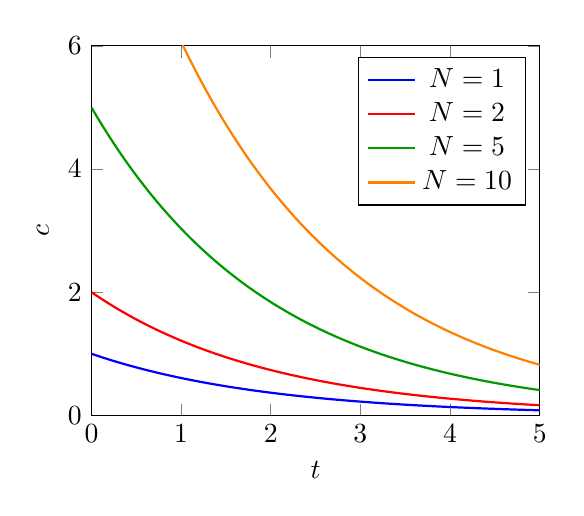
\begin{tikzpicture}
\begin{axis}[xlabel=$t$, ylabel=$c$, xmin=0, xmax=5, ymin=0, ymax=6, width=0.6\textwidth, legend pos=north east]
% Contour curves N(t,c)=k => c = k e^{-0.5 t}
\addplot[blue, thick, domain=0:5, samples=200] {1*exp(-0.5*x)}; \addlegendentry{$N=1$}
\addplot[red, thick, domain=0:5, samples=200] {2*exp(-0.5*x)}; \addlegendentry{$N=2$}
\addplot[green!60!black, thick, domain=0:5, samples=200] {5*exp(-0.5*x)}; \addlegendentry{$N=5$}
\addplot[orange, thick, domain=0:5, samples=200] {10*exp(-0.5*x)}; \addlegendentry{$N=10$}
\end{axis}
\end{tikzpicture}
\end{center}

Answer the following:
\begin{enumerate}
\item According to the level curves, when $c=2$ and $t=0$, the population is $N(0,2) = \answer{2}$.
\item When $c=5$ and $t=2$, the population is $N(2,5) = \answer{5e^{1}} \approx \answer[tolerance=.1]{13.5914}$.
\item Which of the following statements are true? (Select all)
    \begin{selectAll}
        \choice{For fixed $c$, $N$ grows linearly in $t$}
        \choice[correct]{For fixed $c$, $N$ grows exponentially in $t$}
        \choice{For fixed $c$, $N$ decreases with $t$}
        \choice[correct]{For fixed $t$, $N$ is linear in $c$}
        \choice{For fixed $t$, $N$ is exponential in $c$}
    \end{selectAll}
\end{enumerate}



\begin{feedback}
For fixed $c$, $N(t,c)=c e^{0.5t}$ increases exponentially in $t$ (rapid growth). For fixed $t$, $N$ is linear in $c$ (doubling $c$ doubles $N$). Note $N(0,c)=c$, the initial population, and $N(2,5)=5e^{1}\approx 13.5914$.
\end{feedback}
\end{problem}

\section*{Practice and Checking Understanding}

Let's do some practice problems and some quick checks about our visual intuitions.
\begin{problem}
Consider the function $f(x, y) = x^2 + 3xy - y^2$, evaluate:

$$f(2, 1) = (\answer{2})^2 + 3(\answer{2})(\answer{1}) - (\answer{1})^2 = \answer{9}$$

$$f(-1, 2) = (\answer{-1})^2 + 3(\answer{-1})(\answer{2}) - (\answer{2})^2 = \answer{-9}$$

\begin{feedback}
To evaluate $f(x,y)$ at $(a,b)$, substitute $x=a$ and $y=b$. Order matters!
\end{feedback}
\end{problem}

\begin{problem}
Consider the three-variable function $g(x, y, z) = xy + yz + xz$. Evaluate:

$$g(1, 2, 3) = (\answer{1})(\answer{2}) + (\answer{2})(\answer{3}) + (\answer{1})(\answer{3}) = \answer{11}$$

$$g(0, 5, 10) = \answer{50}$$
\end{problem}

Now let's think about some visual intuitions.
\begin{problem}
For two-variable functions $z = f(x,y)$, the graph is:
\begin{multipleChoice}
    \choice{A curve in 2D}
    \choice{A curve in 3D}
    \choice[correct]{A surface in 3D}
    \choice{A volume in 3D}
\end{multipleChoice}

The set $z\leq f(x,y)$ represents:
\begin{multipleChoice}
    \choice{A curve in 2D}
    \choice{A curve in 3D}
    \choice{A surface in 3D}
    \choice[correct]{A volume in 3D}
\end{multipleChoice}

The set $(x,y)$ such that $f(x,y) = 4$ represents:
\begin{multipleChoice}
    \choice[correct]{A curve in 2D}
    \choice{A curve in 3D}
    \choice{A surface in 3D}
    \choice{A volume in 3D}
\end{multipleChoice}

\begin{feedback}
Each point $(x, y)$ gives a height $z = f(x, y)$, creating a surface—like a landscape! If we consider all points below that surface ($z \leq f(x,y)$), we get a volume. Finally, fixing $f(x,y) = 4$ gives a contour line (level curve) in the $xy$-plane.
\end{feedback}
\end{problem}

\begin{problem}
Consider $f(x, y) = x^2 + y^2$. Evaluate at key points: 

$$f(0, 0) = \answer{0}$$  

$$f(1, 1) = \answer{2}$$

$$f(2, 2) = \answer{8}$$

Using MATLAB or some graphing software, this surface resembles:
\begin{multipleChoice}
    \choice{A plane}
    \choice{A saddle}
    \choice[correct]{A paraboloid (bowl) opening upward}
    \choice{A sphere}
\end{multipleChoice}

If you slice the surface horizontally at different $z$-values, the level curves are:
\begin{multipleChoice}
    \choice{Lines}
    \choice{Ellipses}
    \choice[correct]{Circles}
    \choice{Parabolas}
\end{multipleChoice}

\begin{feedback}
Since $f(x,y) = x^2 + y^2 \geq 0$ and increases away from the origin, it forms a bowl (paraboloid).
\end{feedback}
\end{problem}

\begin{problem}
Now consider $g(x, y) = x^2 - y^2$. Evaluate:

$$g(0, 0) = \answer{0}$$

$$g(1, 0) = \answer{1}$$

$$g(0, 1) = \answer{-1}$$

Using MATLAB or graphing software, this surface resembles:
\begin{multipleChoice}
    \choice{A bowl}
    \choice[correct]{A saddle (curves up in one direction, down in another)}
    \choice{A plane}
\end{multipleChoice}

Slicing the surface horizontally at different $z$-values, the level curves are:
\begin{multipleChoice}
    \choice{Circles}
    \choice{Ellipses}
    \choice[correct]{Hyperbolas}
    \choice{Parabolas}
\end{multipleChoice}

\begin{feedback}
The function $g(x,y) = x^2 - y^2$ creates a saddle shape because it curves upward in the $x$-direction and downward in the $y$-direction. The level curves are hyperbolas, reflecting this mixed curvature.
\end{feedback}
\end{problem}

\section*{Extending to More Variables}

\begin{problem}
Functions can have any number of variables! For $f(x, y, z, w)$ of four variables, the domain consists of:

\begin{multipleChoice}
    \choice{Points in 3D space}
    \choice[correct]{Ordered 4-tuples $(x, y, z, w)$}
    \choice{Surfaces in 3D}
\end{multipleChoice}

\begin{feedback}
In machine learning, functions often have thousands of variables. We can't visualize them, but the math works the same!
\end{feedback}
\end{problem}

\begin{problem}
For $h(x, y, z) = x + 2y + 3z$, evaluate:

$h(1, 2, 3) = \answer{1} + 2(\answer{2}) + 3(\answer{3}) = \answer{14}$

$h(-1, 3, 2) = \answer{-1} + 2(\answer{3}) + 3(\answer{2}) = \answer{11}$

\begin{feedback}
Same process: substitute and calculate!
\end{feedback}
\end{problem}

\end{document}
